\section{Elicitation of requirements}
\label{sec:obtainingreq}

The customer did not provide a distinct set of specifications when the project first started. Instead, the team was provided with a general idea and a list of concepts that the customer requested to be included in the app. These concepts are shown as a set of prioritized steps in figure~\ref{fig:roadmap}. It was up to the team to map out a preliminary list of features that could later be approved in cooperation with the customer.

\begin{figure}[H]
\centering
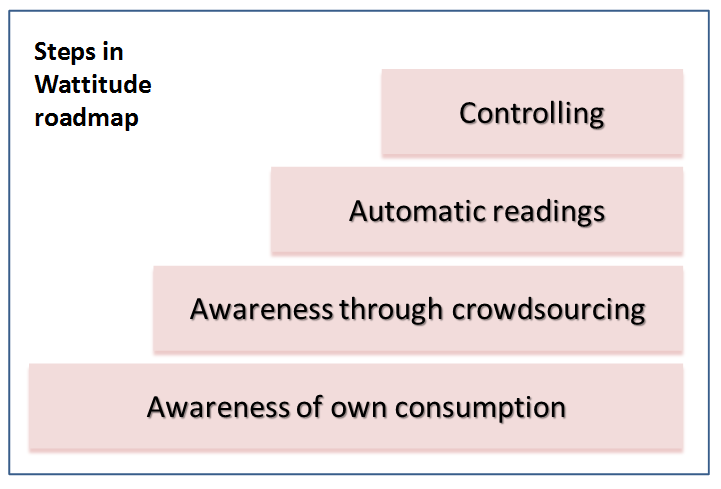
\includegraphics[height=0.4\textheight]{ch/specification/fig/roadmap.png}
\caption{Roadmap for Wattitude functionality}
\label{fig:roadmap}
\end{figure}

Some of these requirements were:
\begin{itemize}
\item The app should be user friendly and simple, so that anyone could measure their energy consumption. This was to be done preferably per device. 
\item The users should be able to share their energy consumption and production with their friends on Facebook. 
\item The concept of \gls{gamification} should be included into the app by allowing the users to compete with each other on saving and/or producing the most energy. 
\item The finished product should include a user manual and complete technical documentation.
\end{itemize}

\noindent To measure the user's energy consumption per device, the team needed a hardware device. Optimally, such a device transmits  data either via Wifi, Bluetooth, or another form of wireless communication protocol.

Due to time restrictions, the requirement of having hardware monitoring and control over each individual device was deemed optional, and only to be attempted if the team had enough time. After the initial project planning and prestudy, the team realized that this was not the case, and the team agreed with the customer to drop these requirements. 

However, the team agreed to do preliminary research on possible hardware solutions provided by the customer. This was done to ease integration in future development when the customer continues development. See chapter~\ref{sec:further} for more about further development. In addition to the requirements described in section~\ref{sec:functionalReq} and~\ref{sec:nonFunctionalReq}, the customer wanted the team to write a user manual for the app and technical documentation for setting up the server. These can be found in appendix~\ref{sec:userManual} and~\ref{sec:technicalDocumentation}.
\newpage
 
%In addition to the customer's own requirements, the team came up with some suggestions to requirements specifications that were discussed and added in collaboration with the customer. %Further details of the final version of the requirements specification are described in the subsequent sections.
